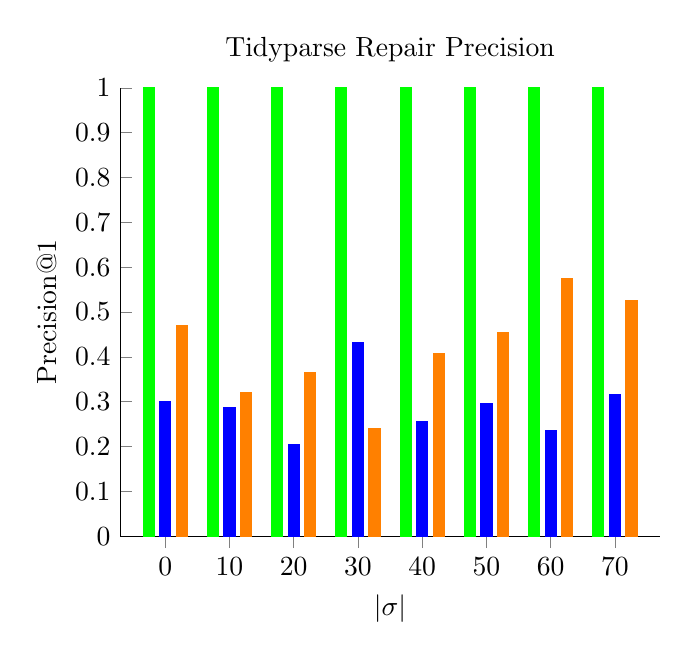
\begin{tikzpicture}
  \begin{axis}[
    xlabel={$|\sigma|$},
    ylabel={Precision@1},
    title={Tidyparse Repair Precision},
    ybar,
    axis lines*=left,
    xtick={0, 10, 20, 30, 40, 50, 60, 70},
    ytick={0, 0.1, 0.2, 0.3, 0.4, 0.5, 0.6, 0.7, 0.8, 0.9, 1.0},
    ymax=1.0,
    ymin=0.0,
    bar width=4pt,
  ]

  \addplot[green, fill=green] coordinates {(0, 1.0) (10, 1.0) (20, 1.0) (30, 1.0) (40, 1.0) (50, 1.0) (60, 1.0) (70, 1.0)};
  \addplot[blue, fill=blue] coordinates {(0, 0.3) (10, 0.286) (20, 0.205) (30, 0.433) (40, 0.256) (50, 0.296) (60, 0.236) (70, 0.315)};
  \addplot[orange, fill=orange] coordinates {(0, 0.46875) (10, 0.321) (20, 0.366) (30, 0.24) (40, 0.407) (50, 0.454) (60, 0.574) (70, 0.526)};

%  \legend{Δ=1,Δ=2,Δ=3}
  \end{axis}
\end{tikzpicture}